
\documentclass[12pt]{article}

\usepackage{scicite}
\usepackage{times}
\usepackage{graphicx}
\usepackage{hyperref}
\usepackage{enumitem}

\topmargin -1.5cm
\oddsidemargin 0.0cm
\textwidth 16cm 
\textheight 23.5cm
\footskip 1.0cm

\newenvironment{sciabstract}{%
\begin{quote} \bf}
{\end{quote}} 

\newcounter{lastnote}
\newenvironment{scilastnote}{%
  \setcounter{lastnote}{\value{enumiv}}%
  \addtocounter{lastnote}{+1}%
  \begin{list}%
  {\arabic{lastnote}.}
  {\setlength{\leftmargin}{.22in}}
  {\setlength{\labelsep}{.5em}}
}
{\end{list}}

\title{Assignment 2} 

\author
{Filipe Pires [85122], João Alegria [85048]\\
\\
Information Retrieval\\
\normalsize{Department of Electronics, Telecommunications and Informatics}\\
\normalsize{University of Aveiro}\\
} 

\date{\today{}}

%%%%%%%%%%%%%%%%% END OF PREAMBLE %%%%%%%%%%%%%%%%

\begin{document} 
\baselineskip18pt
\maketitle 

\section*{Introduction}

This report follows the work delivered for the first assignment of the 
discipline of 'Information Retrieval' and describes both the updates made
on the initial solution and the development of new features related to the
indexing of text corpus.

We include the updates done on each class developed and on the respective
methods, as well as the redesign of our class diagram.
We also provide the instructions on how to run our code.

An explanation on the implementation of the SPIMI approach for the indexing
process that considers memory limitations is presented in this report.
Changes to the output file (the actual index) format are also explained.

Along with the description of the solution, we also answer to a few questions
proposed for the assignment \cite{assign2}.
All code and documentation is present in our public GitHub at 
\newline \url{https://github.com/joao-alegria/RI}. 

\newpage
\section*{1. Updates to Assignment 1}

Once concluded the period of time dedicated for the development of the work 
proposed for the first assignment, a few problems with our delivery were
detected and we found that their solution, although simple, was important to
be presented in this next assignment.

In point d) of the 4th task of assignment 1, it was asked for us to present
the ten terms with highest document frequency according to the index produced
by our program using both tokenizer implementations.
Our mistake was that we presented the ten terms with highest collection 
frequency. To make up for this error, we decided to present here the ten terms
with highest document frequency, as well as those with highest collection 
frequency and those with highest term frequency.
The difference between these 3 statistical properties are presented below:

\begin{itemize}[leftmargin=*]
\setlength\itemsep{-0.3em}
\item Document Frequency - the number of documents in a collection where 
a given token occurs.
\item Term Frequency - the number of occurrences of a given token in a 
document.
\item Collection Frequency - the total number of occurrences of a given 
token in the collection.
\end{itemize}

The 10 terms with highest document frequency (for both tokenizers) are the 
following:

\begingroup
\addtolength\leftmargini{-0.4in}
\addtolength\baselineskip{-0.05in}
\begin{quote}
\begin{verbatim}
Simple:
Terms: 'and' (1739514), 'the' (1589467), 'with' (598916), 
'for' (585442), 'from' (229502), 'patients' (226388), 
'human' (211802), 'cell' (171278), 'cells' (167779), 
'study' (167384).

Complex:
Terms: 'cell' (323874), 'patient' (284668), 'effect' (279130),
'human' (226069), 'studi' (215412), 'activ' (192730),
'use' (176649), 'protein' (175199), 'rat' (171824),
'diseas' (165580).
\end{verbatim}
\end{quote}
\endgroup

The 10 terms with highest term frequency (for both tokenizers) are the 
following:

\begingroup
\addtolength\leftmargini{-0.4in}
\addtolength\baselineskip{-0.05in}
\begin{quote}
\begin{verbatim}
Simple:
Terms: ['the'] (14), ['alpha','ucdeq'] (12), ['mcm'] (11),
['and','eta','mcma','nov','nvheq','sorbitan','tky'] (10).

Complex:
Terms: ['alpha'] (11), ['eta','nov','sarcosin','sorbitan'] (10),
['edta','failur','kinas','manp'] (9), ['beta','buttiauxella',
'hla','mycoplasma','placent','pseudomona', 'silic','subsp',
'tick','val'] (8).
\end{verbatim}
\end{quote}
\endgroup

The 10 terms with highest collection frequency (for both tokenizers) are the 
following:

\begingroup
\addtolength\leftmargini{-0.4in}
\addtolength\baselineskip{-0.05in}
\begin{quote}
\begin{verbatim}
Simple:
Terms: 'and'(2044099), 'the'(2033707), 'with'(633062), 
'for'(608296), 'from'(234101), 'patients'(228824),
'human'(217457), 'cell'(184034), 'cells'(174998),
'study'(170588)

Complex:
Terms: 'cell'(359036), 'patient'(289130), 'effect'(281633),
'human'(232049), 'studi'(219451), 'activ'(202904),
'protein'(188952), 'use'(178166), 'rat'(173397),
'diseas'(169893)
\end{verbatim}
\end{quote}
\endgroup

Let us now take a look at the updates made for the purpose of this second 
assignment.

The first update we made to our code was on the content of the index files 
produced by our indexer. Initially it would write to a text file a token
per line followed by a comma (',') and all document IDs of the documents that
contained the respective token, paired with the respective frequency (with
a ':' between each docID and frequency value).
For this assignment, we altered this format in order to store the position
of each occurrence and the term frequency weight (tfw) and inverse document 
frequency (idf) of each term, following the given format:

\begingroup
\addtolength\leftmargini{-0.4in}
\begin{quote}
\begin{verbatim}
token:idf, docID:tfw:pos1,pos2,...; docID:tfw:...; ...
\end{verbatim}
\end{quote}
\endgroup

Actually, we implemented this in such way that it is possible for the user
to choose from 4 different combinations of output formats, varying the 
presentation of either the frequency or the weight and the presentation or
not of the positions of the terms in each document.
Although this was not specifically asked in the assignment instructions,
it answers its requirements and gives the user a wider range of usage 
alternatives. 

Regarding the structure of our abstract classes, a few changes had to be
considered to better face the challenges of the second assignment.
These, however, were not very relevant in terms of difficulty or time
consumption.

The capacity of regulating the amount of memory used during the program's
execution was a more complex task, with several aspects that required close
attention. Our work on the implementation of a SPIMI approach is explained
in detail further ahead, but it is good to mention that a few updates to 
the {\it main()\/} function had to be made in order for this and all other 
changes to be supported by the new version of the program.
Still on the updates to the initial phases of the program execution, it is
important to mention that we altered the way we process the arguments passed
to the scripts when running them. The changes were made to employ the standard
form of dealing with script parameters, with the help of the \texttt{getopt}
Python library \cite{getopt}.

\section*{2. Architecture \& Memory Usage}

The remaining of the report supposes that the reader has knowledge about what
was presented on the first delivery. 
We will only explain the structure of new components not yet seen by the reader 
and the updates made on the class diagram.

In this chapter we also get into deeper detail on how is memory usage
considered, as well as on how are the new attributes such as the term weights 
calculated and stored.
Figure \ref{fig:classdiagram} shows the new class diagram, with a considerable
increase in complexity compared to the initial version.

\begin{figure}[h!]
  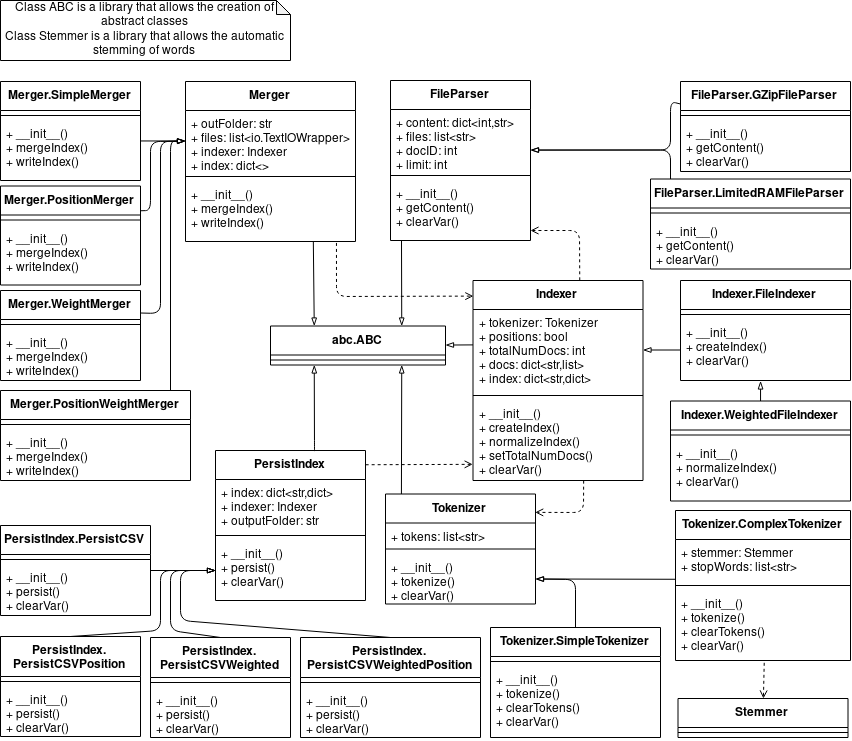
\includegraphics[width=\linewidth]{ClassDiagram_assign2.png}
  \caption{Program's class diagram.}
  \label{fig:classdiagram}
\end{figure}

First of all, we have the new class derived from \texttt{FileParser} with the
name \texttt{LimitedRAM} \texttt{FileParser}. This class does the same as its 
"sister" \texttt{GZipFileParser}, except that \textit{getContent()} is now 
called 1 time per document and returns the information relative to that 
document only. 
Although this makes the reading process slower, it also drastically 
reduces the amount of RAM required during execution.

The \texttt{WeightedFileIndexer} is a new class derived from our \texttt{FileIndexer}.
This class inherits the method \textit{createIndex()} from our previous implementation
and makes use of the method \textit{normalizeIndex()} to calculate the term frequencies.
We call it a normalization as it is a transformation of the produced index to standardize
its values according to a set of rules.
We calculate the term frequencies following the logarithmic formula and the process of 
normalization is based on the cosine formula, both presented bellow.

....... ...... ........... ......... ........... ............. .............. ......

The \texttt{Tokenizer} implementations were the only classes that suffered no changes nor
recieved no new subclasses. 
Our solution served perfectly for the tokenization process whether the program is executed
with a memory limitation or not.

For the \texttt{PersistIndex} class, we developed 3 new classes derived from it - one for
each new output format. 
Following are small portions of indexes generated by our solution in the formats supported
by the program, for analysis purposes.

...... .......... ............ ............ ............ .... ....... .........

We now proceed to explaining how was the memory considered in this second assignment and,
more specifically, what is the SPIMI strategy already mentioned in this document.

// explain the implementation of SPIMI
while memory available:
  fileparser le document
  indexer recebe-o e adiciona index interno (com ajuda do tokenizer)
  if memory limit
    indexer normaliza index
    persister recebe index e posicao (posicao de ocorrencia dos termos)
    persister escreve n1 ficheiro temporario (intermediate\_index\_x)
    clear memory
..............................

\newpage
\section*{3. Index Merging}


// ..............................

\newpage
\section*{4. Discussion}

To test the capabilities of the developed software, we indexed the same
2 large compressed files used on the previous deliver, with the names 
\texttt{2004\_TREC\_ASCII\_MEDLINE\_1.gz} and 
\texttt{2004\_TREC\_ASCII\_MEDLINE\_2.gz}.
Their structure, as collections (corpus) of documents, remained the same.
In this chapter we discuss our implementation's efficiency over these 
files according to the following measures:

a) What is the total indexing time and final index size on disk?

b) What is the maximum amount of memory used during indexing?

// ................................

\newpage
\section*{Conclusions}

After completing the assignment, we drew a few conclusions regarding our
solutions and the whole concept of memory management and its balancing with
good efficiency.

// ...................................

\begin{thebibliography}{9}
  \bibliographystyle{Science}

  \bibitem{assign2}
    S. Matos,
    \textit{IR: Assignment 2},
    University of Aveiro,
    2019/20.
  \bibitem{getopt}
    GetOpt Library - C-Style Parser for Command Line Options,
    Python.org
    \textit{https://docs.python.org/2/library/getopt.html},
    (visited in 25/10/2019)
  
\end{thebibliography}

\clearpage

\end{document}




















